\section{Persistence Diagrams}
\label{section-diagrams}

In this section we define the diagram of a persistence module over $\R$, generalising the barcode of standard persistent homology. If a persistence module $\V$ is decomposable into interval modules, we can use the obvious definition: the multiset in $\R^2$ with a point at $(p, q)$ for each interval $\I(p^*, q^*)$. When $\V$ does \emph{not} decompose into interval modules, we will have to work a little harder.

The strategy is as follows. To every persistence module over $\R$ we associate an `r-measure': a function that assigns every rectangle in $\R^2$ an integer measure. We then show there is a bijection between the appropriate classes of r-measures and multisets in $\R^2$.

\subsection{Abstract r-measures}

First we define r-measures and derive some of their basic properties.

\begin{definition}
Let $\mathcal{D}$ be a subset of $\R^2$. We define $\Rect(\mathcal{D})$ to be the set of closed rectangles lying inside $\mathcal{D}$, i.e., 
\begin{align*}
\Rect(\mathcal{D}) = \{ [a, b] \times [c, d] \subset \mathcal{D} \st a < b \text{ and } c < d \}
\end{align*}
An \emph{r-measure} on $\mathcal{D}$ is a function $\mu : \Rect(\mathcal{D}) \to \{0, 1, 2, \dots \} \cup \{\infty\}$ that is additive under horizontal and vertical splits:
\begin{align*}
\mu([a, b] \times [c, d]) &= \mu([a, p] \times [c, d]) + \mu([p, b] \times [c, d])\\
\mu([a, b] \times [c, d]) &= \mu([a, b] \times [c, q]) + \mu([a, b] \times [q, d])
\end{align*}
for $a < p < b$ and $c < q < d$. Figure~\ref{fig:rmeasure} shows how to interpret these equations pictorially.

\begin{figure}[!htb]
\centering
\begin{tabular}{c c c c}
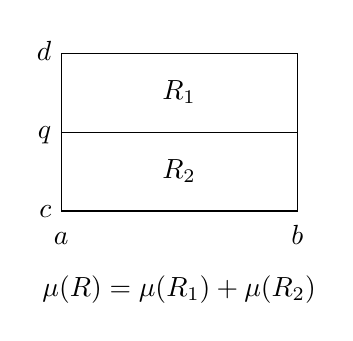
\begin{tikzpicture}[scale=2]
  \coordinate (a) at (0,0);
  \coordinate (b) at (1.5, 0);
  \coordinate (c) at (1.5, 1);
  \coordinate (d) at (0, 1);
  
  \draw (a) rectangle (c);
  \path[draw] (0, 0.5) -- (1.5, 0.5);
  
  \draw (0.75,0.25) node {$\strut{R_2}$};  
  \draw (0.75,0.75) node {$\strut{R_1}$};    
  
  \draw (0,0) node[left] {$\strut{c}$};
  \draw (0,0.5) node[left] {$\strut{q}$};
  \draw (0,1) node[left] {$\strut{d}$};
  
  \draw (0,0) node[below] {$\strut{a}$};
  \draw (1.5,0) node[below] {$\strut{b}$};
  
  \draw (0.75, -0.5) node {$\mu(R) = \mu(R_1) + \mu(R_2)$};  
\end{tikzpicture} & & &
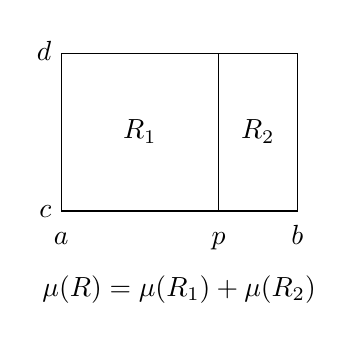
\begin{tikzpicture}[scale=2]
  \coordinate (a) at (0,0);
  \coordinate (b) at (1.5, 0);
  \coordinate (c) at (1.5, 1);
  \coordinate (d) at (0, 1);
  
  \draw (a) rectangle (c);
  \path[draw] (1, 0) -- (1, 1);
  
  \draw (0.5,0.5) node {$\strut{R_1}$};  
  \draw (1.25,0.5) node {$\strut{R_2}$};    
  
  \draw (0,0) node[left] {$\strut{c}$};
  \draw (0,1) node[left] {$\strut{d}$};
  
  \draw (0,0) node[below] {$\strut{a}$};
  \draw (1,0) node[below] {$\strut{p}$};
  \draw (1.5,0) node[below] {$\strut{b}$};
  
  \draw (0.75, -0.5) node {$\mu(R) = \mu(R_1) + \mu(R_2)$};  
\end{tikzpicture}
\end{tabular}
\caption{Horizontal and vertical splitting for r-measures}
\label{fig:rmeasure}
\end{figure}
\end{definition}

We will see that r-measures have many of the features of ordinary measures when restricted appropriately to rectangles in the plane.

\begin{proposition}[Finite additivity]
Let $\mu$ be an r-measure on $\mathcal{D}$. If a rectangle $R$ can be written as a union $R = R_1 \cup \dots \cup R_k$ of rectangles with disjoint interiors, then $\mu(R) = \mu(R_1) + \dots + \mu(R_k)$.
\end{proposition}
\begin{proof}
Let $R = [a, b] \times [c, d]$. By the vertical splitting property, the statement holds for any decomposition $R_i = [a_i, a_{i+1}] \times [c, d]$ with $a = a_1 < a_2 < \dots < a_n = b$. Similarly, by the horizontal splitting property, the statement holds for $R_i = [a, b] \times [c_j, c_{j+1}]$. with $c = c_1 < c_2 < \dots < c_m = d$.

By performing both types of splits, it follows that finite additivity holds for any `product' decomposition of the form $R_{ij} = [a_i, a_{i+1}] \times [c_j, c_{j+1}]$. Now for an arbitrary decomposition $R = R_1 \cup \dots \cup R_k$, decompose each component $R_i$ into the above form, so the entire decomposition also has the form of a `product'. The result follows.
\end{proof}

\begin{proposition}[Monotonicity]
If $R \subseteq S$ then $\mu(R) \leq \mu(S)$.
\end{proposition}
\begin{proof}
This follows from the above proposition, as $S$ must have a decomposition containing $R$ as a component. This can always be done with at most nine rectangles using the coordinates of $R$ as the locations of the splits, as suggested by Figure~\ref{fig:monotonicity}. Then:
\begin{align*}
\mu(S) &= \mu(R) + \mu(R_1) + \dots\\
&\geq \mu(R).
\end{align*}

\begin{figure}[!htb]
\centering
\begin{tikzpicture}[scale=3]
  \coordinate (a) at (0,0);
  \coordinate (b) at (1.5, 0);
  \coordinate (c) at (1.5, 1);
  \coordinate (d) at (0, 1);
  
  \coordinate (a') at (0.25, 0.25);
  \coordinate (c') at (1, 0.75);  
  
  \draw (a) rectangle (c);
  \draw[dashed] (0.25, 0) -- (0.25, 1);
  \draw[dashed] (1, 0) -- (1, 1);
  \draw[dashed] (0, 0.25) -- (1.5, 0.25);
  \draw[dashed] (0, 0.75) -- (1.5, 0.75);

  \draw (a') rectangle (c');
  
  \draw (0.62, 0.5) node {$\strut{R}$};
  \draw (0, 0.5) node[left] {$\strut{S}$};
\end{tikzpicture}

\caption{Splitting used in the proof of monotonicity}
\label{fig:monotonicity}
\end{figure}
\end{proof}

\begin{proposition}[Subadditivity]
If $R \subseteq R_1 \cup \dots \cup R_n$ then $\mu(R) \leq \mu(R_1) + \dots + \mu(R_n)$.
\end{proposition}
\begin{proof}
Let $\{a_i\}$ be the $x$-coordinates of the corners of every rectangle, and $\{c_j\}$ the $y$-coordinates. Subdivide every rectangle into tiles of the form $[a_i, a_{i+1}] \times [c_j, c_{j+1}]$. Every tile that comprises $R$ must belong to some $R_i$ and the result follows by additivity.
\end{proof}

\subsection{The persistence measure}

From any persistence module $\V$, we construct an r-measure that `counts' the points of the barcode of $\V$ that fall inside each rectangle. We can use this r-measure to construct a persistence diagram for \emph{any} persistence module, not only those that decompose into intervals.

Let $\H$ be the half-plane in $\R^2$ given by:
\begin{align*}
\H = \{ (p, q) \st p \leq q \}
\end{align*}

\begin{definition}
The \emph{persistence measure} of $\V$ is the function
\begin{align*}
\mu_\V(R) = \langle \qoff{a} \qem \qon{b} \qem \qon{c} \qem \qoff{d} \st \V \rangle,
\end{align*}
for any $R = [a, b] \times [c, d]$ with $a < b \leq c < d$.
\end{definition}

\begin{proposition}
$\mu_\V$ is a r-measure on $\H$.
\end{proposition}
\begin{proof}
We must show that $\mu_\V$ is additive under horizontal and vertical splitting. For horizontal splitting, let $a < p < b \leq c < d$. Then, by the restriction principle,
\begin{align*}
\mu_\V([a, b] \times [c, d]) &= \langle \qoff{a} \qem \qno \qem \qon{b} \qem \qon{c} \qem \qoff{d} \st \V \rangle\\
&= \langle \qoff{a} \qem \qon{p} \qem \qon{b} \qem \qon{c} \qem \qoff{d} \st \V \rangle + \langle \qoff{a} \qem \qoff{p} \qem \qon{b} \qem \qon{c} \qem \qoff{d} \st \V \rangle \\
&= \langle \qoff{a} \qem \qon{p} \qem \qno \qem \qon{c} \qem \qoff{d} \st \V \rangle + \langle \qno \qem \qoff{p} \qem \qon{b} \qem \qon{c} \qem \qoff{d} \st \V \rangle \\
&= \mu_\V([a, p] \times [c, d]) + \mu_\V([p, b] \times [c, d]).
\end{align*}

For vertical splitting, let $a < b \leq c < q < d$, then:
\begin{align*}
\mu_\V([a, b] \times [c, d]) &= \langle \qoff{a} \qem \qon{b} \qem \qon{c} \qem \qno \qem \qoff{d} \st \V \rangle\\
&= \langle \qoff{a} \qem \qon{b} \qem \qon{c} \qem \qoff{q} \qem \qoff{d} \st \V \rangle + \langle \qoff{a} \qem \qon{b} \qem \qon{c} \qem \qon{q} \qem \qoff{d} \st \V \rangle  \\
&= \langle \qoff{a} \qem \qon{b} \qem \qon{c} \qem \qoff{q} \qno \qem  \st \V \rangle + \langle \qoff{a} \qem \qon{b} \qem \qno \qem \qon{q} \qem \qoff{d} \st \V \rangle \\
&= \mu_\V([a, b] \times [c, q]) + \mu_\V([a, b] \times [q, d]).
\end{align*}
\end{proof}

Let us consider the simplest case: when $\V$ is an interval module $\I^J$ for some $J = (p^*, q^*)$. Let $R = [a, b] \times [c, d]$ be a rectangle, then $\mu_\V(R)$ is determined as follows. The restriction of $\I^J$ to the indexing set $\T = \{a, b, c, d\}$ is clearly either an interval or zero. Therefore, $\mu_\V(R)$ is equal to either 0 or 1. $\mu_\V(R) = 1$ precisely when $\I^J_\T = \qoff{a} \qem \qon{b} \qem \qon{c} \qem \qoff{d}$, i.e., $[b, c] \subseteq J \subseteq (a, d)$.

Using the notation for extended real numbers, this condition is equivalent to $a^+ \leq p^* \leq b^- \leq c^+ \leq q^* \leq d^-$. This relationship is easiest to explain pictorially. We represent an interval $(p^*, q^*)$ as the point $(p, q) \in \R^2$, with a tick to indicate the annotations. For example, the point $(p^+, q^+)$ has a tick towards the upper right. Figure~\ref{fig:decoratedpoints} demonstrates this representation.

The intervals $(p^*, q^*)$ that are `detected' by the rectangle $R$ are precisely the intervals whose point $(p, q)$ \emph{and} tick mark are contained in $R$. We abuse notation and say $(p^*, q^*) \in R$ when the interval $J = (p^*, q^*)$ satisfies $[b, c] \subseteq J \subseteq (a, d)$ as above. The points shown in Figure~\ref{fig:decoratedpoints} are examples of points `contained' in a rectangle $R$.

\begin{figure}[!htb]
\centering
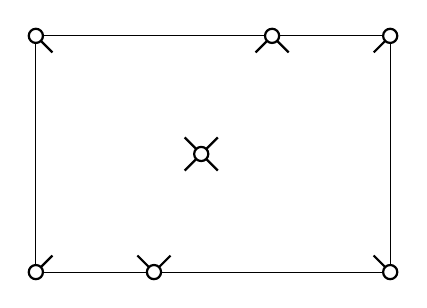
\begin{tikzpicture}[scale=3]
  \coordinate (a) at (0,0);
  \coordinate (b) at (1.5, 0);
  \coordinate (c) at (1.5, 1);
  \coordinate (d) at (0, 1);
  
  \draw (a) rectangle (c);

  \draw[thick] (a) -- (0.07, 0.07);
  \draw[thick, fill=white] (a) circle (0.03);
  
  \draw[thick] (1.5, 1) -- (1.43, 0.93);
  \draw[thick, fill=white] (c) circle (0.03);  

  \draw[thick] (0, 1) -- (0.07, 0.93);
  \draw[thick, fill=white] (0, 1) circle (0.03);  
  
  \draw[thick] (1.5, 0) -- (1.43, 0.07);
  \draw[thick, fill=white] (1.5, 0) circle (0.03);    
  
  \draw[thick] (0.5, 0) -- (0.57, 0.07);
  \draw[thick] (0.5, 0) -- (0.43, 0.07);
  \draw[thick, fill=white] (0.5, 0) circle (0.03);
  
    \draw[thick] (1, 1) -- (0.93, 0.93);
  \draw[thick] (1, 1) -- (1.07, 0.93);
  \draw[thick, fill=white] (1,1) circle (0.03);
  
  \draw[thick] (0.7, 0.5) -- (0.77, 0.57);
  \draw[thick] (0.7, 0.5) -- (0.63, 0.57);
  \draw[thick] (0.7, 0.5) -- (0.77, 0.43);
  \draw[thick] (0.7, 0.5) -- (0.63, 0.43);
  \draw[thick, fill=white] (0.7, 0.5) circle (0.03);
\end{tikzpicture}
\caption{Some decorated points `detected' by $R$}
\label{fig:decoratedpoints}
\end{figure}

When $\V$ is decomposable, $\mu_\V$ is easy to describe.

\begin{proposition}
\label{prop-decomposable-diagram}
Let $V = \bigoplus \I^{l_i}$ be a decomposable persistence module with intervals $\{ l_i \}$. Then
\begin{align*}
\mu_\V(R) = \left | \{ l_i \st l_i \in R \} \right |
\end{align*}
\end{proposition}
\begin{proof}
This follows from the discussion above and Proposition~\ref{quiver-direct-sums}.
\end{proof}

\subsection{Equivalence}

We now have a mechanism to pass from persistence modules to r-measures. In this section we show that every finite r-measure uniquely determines a multiset of decorated points.

\begin{definition}
The \emph{r-interior} of a region $\mathcal{D} \subseteq \R^2$ is the set of decorated points:
\begin{align*}
\mathcal{D}^\rint = \{ (p^*, q^*) \st \text{there exists } R \in \Rect(\mathcal{D}) \text{ with } (p^*, q^*) \in R \}.
\end{align*}
\end{definition}

The r-interior of a region is all the points that are `detected' by an r-measure on that region. For example, the upper half plane $\mathcal{H} = \{ (p, q) \st p \leq q \}$ has r-interior:
\begin{align*}
\mathcal{H}^\rint = \{ (p^*, q^*) \st p < q \} \cup \{ (p^-, p^+) \st p \in \R \}.
\end{align*}

\begin{theorem}[Equivalence]\label{r-measure-equivalence}
Let $\mathcal{D} \subseteq \R^2$. There is a bijection between 
\begin{itemize}
\item r-measures on $\mathcal{D}$ such that $\mu(R) < \infty$ for every $R \in \Rect(\mathcal{D})$; and
\item multisets of decorated points $\mathsf{A}$ in $\mathcal{D}^\rint$ such that $\card(\mathsf{A}|_R) < \infty$ for every $R \in \Rect(\mathcal{D})$,
\end{itemize}
where the measure corresponding to a multiset $\mathsf{A}$ is given by the formula
\begin{align*}
\mu(R) = \card(\mathsf{A}|_R).
\end{align*}
\end{theorem} 

The proof of this theorem occupies the remainder of this section. 

\begin{proof}
One direction of the bijection is easy. Given a multiset $\mathsf{A}$, we define $\mu$ as above. We need only verify that the formula above defines an r-measure. Given any horizontal or vertical split $R = R_1 \cup R_2$, any decorated point $(p^*, q^*) \in R$ belongs to exactly one of $R_1$ and $R_2$. Therefore:
\begin{align*}
\mu(R) = \card(\mathsf{A}|_R) = \card(\mathsf{A}|_{R_1}) + \card(\mathsf{A}|_{R_2}) = \mu(R_1) + \mu(R_2).
\end{align*}

Now for the reverse direction. For an r-measure $\mu$, let $\mathsf{A}$ be the multiset in $\mathcal{D}^\rint$ given by the multiplicity function:
\begin{align*}
m(p^*, q^*) = \min \{ \mu(R) \st R \in \Rect(\mathcal{D}), \, (p^*, q^*) \in R \}.
\end{align*}
This is well defined by the well ordering principle, as each $\mu(R)$ is a non-negative integer.

We must prove that $\mathsf{A}$ satisfies the formula in the statement of the theorem and show that it is the unique such multiset. From above, we know that the multiset $\mathsf{A}$ defines an r-measure $\nu$ via:
\begin{align*}
\nu(R) = \card(\mathsf{A}|_R).
\end{align*}
We now show that $\mu = \nu$ by induction on $\mu(R)$, which is finite by the conditions of the theorem.

In the base case, consider all $R$ such that $\mu(R) = 0$. Let $(p^*, q^*)$ be a point contained in one such $R$. Then:
\begin{align*}
0 \leq m(p^*, q^*) \leq \mu(R) = 0.
\end{align*}
Therefore $m(p^*, q^*) = 0$ inside $R$, and $\nu(R) = \mu(R) = 0$.

Now assume that $\mu(R) = \nu(R)$ for every $R$ with $\mu(R) < k$. We must now show that for any rectangle $R_0$ with $\mu(R_0) = k$, also $\nu(R_0) = k$. Split $R_0$ into four equal quadrants $Q_1, Q_2, Q_3, Q_4$. By finite additivity, we have:
\begin{align*}
\mu(R) &= \mu(Q_1) + \mu(Q_2) + \mu(Q_3) + \mu(Q_4) \\
\nu(R) &= \nu(Q_1) + \nu(Q_2) + \nu(Q_3) + \nu(Q_4).
\end{align*}

If more than one of $\mu(Q_i)$ is non-zero, then $\mu(Q_i) < k$ for all $i$, and the result follows by induction. In the remaining case, there is a single quadrant with measure $k$ and the remainder have measure $0$. Let $R_1$ be this distinguished quadrant.

We now repeat the argument with $R_1$. Either we find the quadrants satisfy $\mu(Q_i) < k$ or there is another quadrant with $\mu(Q_i) = k$. The only unhandled case is when we find an infinite sequence of rectangles $R_0 \supset R_1 \supset \dots$ with $\mu(R_i) = k$ for all $i$. The diameters of the quadrants tend to zero, so the intersection $\bigcap R_i$ contains a single point $(r, s)$.

Therefore, the only contribution to $\nu(R)$ must come from decorated points that belong to all the $R_i$, i.e., decorated points of the form $(r^*, s^*)$. Assume for now that $(r, s)$ lies on the interior of every $R_i$. Divide each $R_i$ into quadrants $R_i^{++}, R_i^{-+}, R_i^{+-}, R_i^{--}$ sharing $(r, s)$ as a common corner, and such that $(r^+, s^+)$ lies in $R_i^{++}$ for all $i$, $(r^-, s^+)$ lies in $R_i^{-+}$, and so on.

The result follows from the following claim: Let $(\varepsilon_i)$ and $(\eta_i)$ be non-increasing sequences of positive real numbers that converge to $0$. Then:
\begin{align*}
m(r^+, s^+) = \lim_{i\to\infty} \mu([r, r+\varepsilon_i] \times [s, s+\eta_i]).
\end{align*}

To see that this is true, let $R$ be a rectangle that contains $(r^+, s^+)$. Then for $i$ sufficiently large, $R_i \subseteq R$. By monotonicity, $\mu(R_i)$ must eventually stabilise to a finite limit. Then:
\begin{align*}
m(r^+, s^+) \leq \min \mu(R_i) = \lim_{i \to \infty} \mu(R_i) \leq \mu(R).
\end{align*}
Now, taking the minimum over all $R$, the RHS becomes $m(r^+, s^+)$ and we have the equality we require.

Returning to the proof of the theorem, we have $m(r^+, s^+) = \lim_{i\to\infty} \mu(R_i^{++})$, with the sequence eventually stabilising at this value. We also have the obvious equivalent statements for the remaining decorated points $(r^*, s^*)$. 

For sufficiently large $i$, we therefore have:
\begin{align*}
\nu(R_0) &= m(r^+, s^+) + m(r^+, s^-) + m(r^-, s^+) + m(r^-, s^-) \\
&= \mu(R_i^{++}) + \mu(R_i^{-+}) + \mu(R_i^{+-}) + \mu(R_i^{--}) = \mu(R_i) = k.
\end{align*}

If $(r, s)$ does not lie in the interior of every $R_i$ then beyond some $N$, the point $(r, s)$ lies on the boundary of $R_i$ for all $i > N$. We then have fewer cases to consider: if $(r, s)$ is on an edge then only two decorated points of the form $(r^*, s^*)$ lie in every $R_i$. If $(r, s)$ is on a corner then only one decorated point needs to be considered. In either case, the above argument goes through.

By induction, we have $\mu(R) = \nu(R)$ for every rectangle $R$. All that remains is to show uniqueness. Let $\mathsf{B}$ be some other multiset with associated r-measure $\nu'$ such that $\mu = \nu'$. We must show that $\mathsf{A} = \mathsf{B}$.

Let $m'(p^*, q^*)$ be the multiplicity function for $\mathsf{B}$, and consider any point $(p^*, q^*) \in \mathcal{D}^\rint$. Let $R$ be a rectangle with $(p^*, q^*)$ at a corner. Because $\nu(R) = \nu'(R) = \mu(R) < \infty$, we can choose a rectangle such that $(p^*, q^*)$ is the only point with positive multiplicity in $R$. Then:
\begin{align*}
m(p^*, q^*) = \nu(R) = \mu(R) = \nu'(R) = m'(p^*, q^*).
\end{align*}
Therefore $m = m'$ for all $(p^*, q^*) \in \mathcal{D}^\rint$ and $\mathsf{A} = \mathsf{B}$.
\end{proof}

The theorem leads to the following definitions.

\begin{definition}
The \emph{decorated diagram} $\Dgm(\V)$ of a persistence module $\V$ is the unique multiset of decorated points such that:
\begin{align*}
\mu_\V(R) = \card(\Dgm(\V)|_R)
\end{align*}

If we forget the topology of the `intervals' we have the \emph{undecorated diagram} $\dgm(\V)$. This is a multiset of ordinary points in $\mathcal{D}$ defined by:
\begin{align*}
\dgm(\V) = \{ (p, q) \st (p^*, q^*) \in \Dgm(\V) \} \cap \text{int } \mathcal{D}
\end{align*}
where `$\text{int } \mathcal{D}$' denotes the ordinary interior of $\mathcal{D}$.
\end{definition}

Proposition~\ref{prop-decomposable-diagram} implies that for any persistence module $\V$ that decomposes into interval modules, $\Dgm(\V)$ is precisely the set of intervals in the decomposition.

\subsection{q-tame persistence modules}

The stability theorem of later sections requires a condition on the structure maps of the persistence modules. This condition is quite natural and is satisfied in practical applications, as demonstrated by the theorems of this section.

\begin{definition}
A persistence module is \emph{q-tame} if for any $s < t$, the structure map $v_s^t$ has finite rank.
\end{definition}

Such modules are called `q-tame' because, for any infinite quadrant $[-\infty, b] \times [c, +\infty]$ we have:
\begin{align*}
\mu_\V([-\infty, b] \times [c, +\infty]) = \langle \qon{b} \qem \qon{c} \st \V \rangle = \rank v_b^c < \infty.
\end{align*}

Note that q-tameness does not mean there are no limit points in the persistence diagram, as we may have limit points on the diagonal $\Delta = \{(x, x) \st x \in \R \}$. By limit point, we mean a point such that every neighbourhood of that point contains infinitely many other points.

\begin{example}
The module
\begin{align*}
\V = \bigoplus_{n=1}^\infty \I[0, \tfrac{1}{n}]
\end{align*}
is q-tame with $\dgm(\V) = \{ (0, \tfrac{1}{n}) \st n \geq 1 \}$. This has an limit point at $(0, 0)$.
\end{example}

We now give some examples of how q-tame modules occur in the wild. Our original motivation for studying persistence modules was to understand persistent homology in the setting of finite simplicial complexes. The results in the remainder of this work apply as a result of the following theorem.

\begin{theorem}
\label{thm-simplicial-qtame}
Let $X$ be the geometric realisation of a finite simplicial complex, and $f : X \to \mathbb{R}$ a continuous function. Then the persistence module $H(X^f)$ induced by the sublevelset filtration of $X$ is q-tame.
\end{theorem}
\begin{proof}
Let $X^a$ denote the sublevel set $X^a = f^{-1}((-\infty, a])$. We must show that, for any $a < b$, $H(X^a) \to H(X^b)$ has finite rank.

Begin with any triangulation of $X$ and repeatedly subdivide the simplices of $X$ until no simplex intersects both $A = f^{-1}(a)$ and $B = f^{-1}(b)$. To see that this is always possible, note that because $X$ is compact and both $A$ and $B$ are closed, $A$ and $B$ are themselves compact. Because $A$ and $B$ are compact subsets of $X$, the function $d(x, B)$ attains a minimum on $A$. This minimum $\varepsilon$ must be nonzero, as $A$ and $B$ are disjoint. We therefore subdivide the simplices until the length of every edge is less than $\varepsilon/2$.

Let $Y$ be the the union of every closed simplex that meets $X^a$. Then $Y$ is a finite simplicial complex, and we have inclusions $X^a \subseteq Y \subseteq X^b$. 

The map $H(X^a) \to H(X^b)$ therefore factorises as $H(X^a) \to H(Y) \to H(X^b)$. Because $Y$ is a finite simplicial complex, $H(Y)$ is finite dimensional and $H(X^a) \to H(X^b)$ has finite rank.
\end{proof}

The Vietoris-Rips complex of a finite set must be a finite simplicial complex, and any simplicial filtration of such a complex leads to a q-tame persistence module. The following theorem shows that a much larger class of metric spaces also lead to a q-tame persistence modules. \cite{chazal2013geometric}

\begin{definition}
A metric space is \emph{totally bounded} if, for any $\varepsilon > 0$, the space can be covered with a finite number of open balls of radius $\varepsilon$.
\end{definition}

Any compact metric space is totally bounded. For any $\varepsilon$, construct the cover with an open ball of radius $\varepsilon$ at every point. By compactness there is a finite subcover which is precisely the cover we require.

\begin{theorem}
\label{thm-tb-qtame}
Let $(X, d_X)$ be a totally bounded metric space. Then the persistence module $H(\mathbf{VR}(X, \alpha))$ is q-tame.
\end{theorem}
\begin{proof}(Outline)
Here we provide a sketch of the proof as the full details are not relevant to the rest of this work. Again we must show that, for any $a < b$, $H(\mathbf{VR}(X, a)) \to H(\mathbf{VR}(X, b))$ has finite rank. Let $\varepsilon = (b-a)/2$. Because $X$ is totally bounded, there is a finite subset $Y \subset X$ such that for any $x \in X$, there is a $y \in Y$ with $d_X(x, y) < \varepsilon / 2$. Let $C$ be some (multivalued) matching between the elements of $X$ and $Y$ so that $d_Y(x, C(x)) \leq \varepsilon / 2$.

Let $\sigma \in \mathbf{VR}(X, a)$, and $\tau \subseteq C(\sigma)$ any finite subset. For any $y, y' \in \tau$ there exist $x, x' \in \sigma$ such that $y \in C(x), y' \in C(x')$ and therefore:
\begin{align*}
d_Y(y, y') \leq d_X(x, x') + \varepsilon \leq a + \varepsilon.
\end{align*}
It follows that $\tau \in \mathbf{VR}(Y, a + \epsilon)$. Symmetrically, for any $\tau \in \mathbf{VR}(Y, a + \epsilon)$, $\sigma' \subseteq C(\tau) \in \mathbf{VR}(X, a + 2 \epsilon)$.

After a little work, this implies the factorisation:
\begin{align*}
H(\mathbf{VR}(X, a)) \to H(\mathbf{VR}(Y, a+\varepsilon)) \to H(\mathbf{VR}(X, a+ 2 \varepsilon)) = H(\mathbf{VR}(X, b)).
\end{align*}
Again, the vector space $H(\mathbf{VR}(Y, a+\varepsilon))$ is finite dimensional so the structure maps all have finite rank.
\end{proof}